\chapter{Implementation}\label{chapter:implementation} \

In Chapter~\ref{chapter:implementation} we will introduce
the methods used to implement the experiments to answer
the research goals. In Section~\ref{section:vqa_training}
we will present how the \ac{qml} models are trained.
Futhermore, in Section~\ref{section:vqa_attacks} the
attack methodology on the \ac{vqa} model will be described. \

\section{Variational Quantum Algorithm Model Training}\label{section:vqa_training} \

In this section we will specify how the \ac{vqa} models
were trained. In Subsection~\ref{subsection:preprocess},
we will describe the dataset preprocessing methodology required
for the training. Later on in Subsection~\ref{subsection:config},
the configuration files utilized by the training pipeline will
be defined. Afterwards, in Subsection~\ref{subsection:noise_injection}
we will present how the noise is injected to the
\ac{qml} models during training and evaluation.
Finally, the developed pipeline for the training will
be presented in Subsection~\ref{subsection:pipeline}. \

\subsection{Datasets Preprocessing}\label{subsection:preprocess} \

In order to reduce the execution time of the model training, all the
datasets mentioned in Section~\ref{section:datasets} were
stored preprocessed. All the datasets but the Plus-Minus dataset
were retrieved using OpenML~\cite{vanschoren_openml_2014}. We
obtained the Plus-Minus dataset by asking for it to the authors of 
~\cite{wendlinger_comparative_2024}. \

The preprocessing methodology encompasses for all the datasets the
removal of data points that are missing at least one feature.
Then, duplicate data points are removed to avoid overemphasizing
these elements and creating a bias in the data distribution. In
case the target labels are non-numeric, we modified them to
represent numerical classes. Finally, all the datasets except
the Iris Flower dataset are normalized per feature using the standard
deviation and rescaled between a range of \(0\) and \(1\). This
is done with Scikit-learn~\cite{pedregosa_scikit-learn_2011}
and its purpose is to prevent feature dominance and to quicken
training convergence. \

There is one last details with regards to the preprocessing
of the datasets. Namely that the majority class from the
\ac{pid} dataset was reduced to obtain a balanced dataset
with regards to the class distribution. \

\subsection{Configuration File}\label{subsection:config} \

The configuration files are essential to the training
pipeline. Its contents define the dataset to be used,
which type of \ac{qml} model is going to be trained,
which noise model will be injected, and some hyperparameters
regarding the \ac{qml} model's architecture. These hyperparameters
are the number of qubits, the number of layers, the number of
classes, the learning rate, the batch size, and the epochs. \

\begin{lstlisting}[language=Python, caption={Example configuration file.}, label=lst:config_file]
  {
    "dataset" : "diabetes",
    "qml_model" : "pqc",
    "noise_model" : "none",
    "num_qubits" : 3,
    "num_layers" : 40,
    "num_classes" : 2,
    "learning_rate" : 0.0005,
    "batch_size" : 16,
    "epochs" : 10
  }
\end{lstlisting}

An example configuration file can be seen in Listing
~\ref{lst:config_file}. This configuration file is given
to the training pipeline. Once the training is finished,
two more fields will be added to the configuration file.
These fields are the model accuracy on the test set and an
\(id\) to help identify the resulting model weights. The
configuration files are helpful to automate the training
and prepare the adversarial attacks on all the trained
\ac{qml} models. The hyperparameters used to train the
models can be found in Table~\ref{tab:hyperparameters}. \

\begin{table}[htpb]
  \centering
  \begin{tabular}{| c | c | c | c | c | c | c |}
    \hline
    Dataset & Qubits & Layers & Classes & Learning Rate & Batch Size & Epochs \\
    \hline
    Iris & 2 & 2 & 2 & 0.05 & 30 & 10 \\
    \hline
    \ac{pid} & 3 & 40 & 2 & 0.005 & 30 & 10 \\
    \hline
    Breast-Cancer & 4 & 40 & 2 & 0.0005 & 16 & 10 \\
    \hline
    Plus-Minus & 8 & 32 & 4 & 0.001 & 50 & 10 \\
    \hline
  \end{tabular}
  \caption[Hyperparameters table.]{Hyperparameters used for the different datasets.}\label{tab:hyperparameters}
\end{table}

\subsection{Noise Injection}\label{subsection:noise_injection} \

The Circuit-Centric ansatz is built upon a combination of 
Pennylane's arbitrary rotation gate \colorbox{inline_gray}{\lstinline|Rot|}
and \colorbox{inline_gray}{\lstinline|CNOT|} gates. In the case
of Pennylane, the \(Rot\) gate is native to the framework, therefore,
there is no need to decompose it into other supported gates.
Nevertheless, if other frameworks or devices are utilized,
the gate decomposition is required and it would modify the resulting
trained model. \

\begin{equation}\label{eq:rot_decomposition}
  \Qcircuit @C=0.4em @R=0.4em {
    & \gate{Rot(\theta_{1},\theta_{2},\theta_{3})} & \gate{N(\epsilon)} & \qw \\
    & \gate{Rot(\theta_{1},\theta_{2},\theta_{3})} & \gate{N(\epsilon)} & \qw
  } \qquad
  \Qcircuit @C=0.4em @R=0.4em {
    & \gate{RZ(\theta_{1})} & \gate{N(\epsilon)} & \gate{RY(\theta_{2})} & \gate{N(\epsilon)} & \gate{RZ(\theta_{3})} & \gate{N(\epsilon)} & \qw \\
    & \gate{RZ(\theta_{1})} & \gate{N(\epsilon)} & \gate{RY(\theta_{2})} & \gate{N(\epsilon)} & \gate{RZ(\theta_{3})} & \gate{N(\epsilon)} & \qw
  }
\end{equation} \

Pennylane's \(Rot(\theta_{1},\theta_{2},\theta_{3})\) gate can be
decomposed in three rotational gates, namely the sequence of
\(R_{Z}(\theta_{1})\), \(R_{Y}(\theta_{2})\), and \(R_{Z}(\theta_{3})\).
If we injected the noise after every gate, the influence of noise on
the quantum circuit would increase almost three times (Eq.
~\ref{eq:rot_decomposition}). Consequently, we manually decompose the
\(Rot\) gate into its three corresponding gates to generate a single
layer in the Circuit-Centric ansatz. This will not only allow for the
pipeline in the future to be expanded and tested with new devices
and frameworks, but also will make the results of the thesis valid
for all of the devices and frameworks. \

In Equation~\ref{eq:rot_decomposition} the gate with the letter \(N\)
simulates the injected noise to the circuit. The type of noise model
to be injected to the \ac{qml} model is provided in the previously
described configuration file. The configuration file must then provide
one of the 6 possible noise models and either the corresponding probability
of noise to occur or the angle miscalibration \(\epsilon\). \

In order to inject noise to a \ac{qml} model we utilize Pennylane's
\colorbox{inline_gray}{\lstinline|transform|} module. We utilize it
in two different ways to create \ac{qml} models either with coherent
or incoherent noise. To simulate coherent noise we create a Pennylane
noise model object that will later on be applied to the quantum circuit.
The noise model is conformed by the addition of \(R_{Y}(\epsilon)\),
\(R_{Z}(\epsilon)\), or \(CRX(\epsilon)\) gates to the noiseless
\(R_{Y}(\theta)\), \(R_{Z}(\theta)\), or \(CNOT\) gates respectively
(where \(\epsilon\) represents the miscalibration angle). On the other
hand, to simulate incoherent noise we insert the noisy operation
depending on its type directly to the quantum circuit's gates.
This means that after every quantum gate noise might occur with
a given probability \(\epsilon\). \

For the incoherent noise \ac{qml} models, the chosen values for the
probability of noise occurring are \(2\%\), \(4\%\), \(6\%\), \(8\%\),
and \(10\%\). These values were chosen to be enough to notice an
influence in the training but not to overwhelm the classifier and
drown down any potential learning from the data. The same reasons
apply to the chosen values for the miscalibration angle for coherent
noise, the values are \(2^{\circ}\), \(4^{\circ}\), \(6^{\circ}\),
\(8^{\circ}\), and \(10^{\circ}\). \

\subsection{Training Pipeline}\label{subsection:pipeline} \

The stepping stones for the training pipeline were presented
in the previous subsections. The pipeline has been created
in order to simplify and automatize the training of the
\ac{qml} models. The pipeline is based on the configuration
files. Each \ac{qml} model requires a configuration file to
be trained, therefore, the amount of configuration files
depends on the number of models to be trained. \

In this thesis we are training \ac{qml} models for \(7\)
datasets, with \(6\) noise types with each one having \(5\)
different miscalibrations or probabilities. Adding up
the \(7\) noiseless models, we end up with \(217\) configuration
files and \ac{qml} models to be trained. Manually creating
the configuration files would take a considerable
amount of time. Therefore, we coded a script to
automatically create the configuration files of a
given dataset. \
% 7 * 6 * 5 = 210 + 7 (noiseless) = 217

After the configuration files have been created,
we can start with the training. Training \(217\)
\ac{qml} models individually is also time consuming.
Thus, we created a script that retrieves all
the configuration files from a specific dataset
and performs the model training. More importantly,
the resulting weights of the model are automatically
saved in conjunction with the modified configuration
files. This serves two purposes. Firstly, we need the model
weights to evaluate their accuracy when performing the
adversarial attacks. Secondly, the pipeline checks
if the model has already been previously trained and
can skip retraining it. Therefore, the automated training
can be interrupted and resumed without losing any information
about the trained models. \

The actual model training is performed by using a training loop
based on the PyTorch Lightning~\cite{falcon_pytorch_2019} workflow.
To enable the Lightning workflow we created a helper file with
utility functions that help train and evaluate the \ac{qml} model.
In this file we define the training, validation and testing steps.
Additionally, we implement helper functions to calculate the 
accuracy and a threshold method to be able to evaluate the \ac{qml}
model. Finally, we define the model architecture based on the
weights, number of target labels to classify and a forward pass. \

The Lightning workflow simplifies and streamlines the training.
Nevertheless, in order to perform the training loop, a small
setup before is required. First of all, based on the configuration
file we retrieve the datasets. If the dataset has already been
fetched, we simply load the preprocessed dataset from the local files.
Later on, we define the \ac{qml} model based on the given hyperparameters.
Moreover, the required weights for training the module are randomly
initialized. \

% TODO: Mention specific hyperparameters / qml model architectures per dataset in a table

Once the preprocessed dataset has been loaded, we divide it into
different sets to facilitate the training loop. For most of
the datasets we have a \(70/30\) split between the training
set and the test set. The test set is stratified according
to the data distribution from the training set. For the
Plus-Minus datasets only \(20\%\) of the dataset
is used for training, as theses datasets are substantially
more computationally demanding than the other datasets. \

The last requirements for the training loop to be prepared are the
loss function and the optimizer used to the adapt the \ac{qml} model. In our
specific case we utilize ADAM, a gradient-based optimizer, as it will
lead to faster convergence than just using a gradient descent. For the
loss function we utilize PyTorch's implementation of the Cross Entropy
Loss, therefore, we interpret the resulting measurements from the
\ac{qml} model similar to a probability distribution.  \

Once everything is set up, we let the \textit{Trainer} module
perform the training of the \ac{qml} model. The \textit{Trainer}
module is responsible for loading the data points in the given
batch number, calculating the loss, and optimizing the \ac{qml}
models weights towards convergence. We also implemented an early
stopping mechanism when the training accuracy reaches \(100\%\)
to avoid overfitting the simpler models. \

With this implemented pipeline it is simple to perform
any further updates. The helping files are modularly
designed to be reused, modified, and updated. Incorporating
new and different types of \ac{qml} models with noise
injection is simple. Furthermore, the chosen noise types
and values can be effortlessly modified and expanded. 
Not only does the pipeline enable the replication of results,
but the creation of new experiments. \

\section{Adversarial Attacks on Variational Quantum Algorithm Model}\label{section:vqa_attacks} \

In this section we will specify how the adversarial
attacks and evaluation are performed. In Subsection
~\ref{subsection:adv_attacks}, we will describe the process
to obtain adversarial examples with the \ac{fgsm} and \ac{pgd}
techniques. Afterwards in Subsection~\ref{subsection:evaluation},
the evaluation procedure of the trained \ac{qml} models against
adversarial examples will be defined. \

\subsection{Adversarial Attacks}\label{subsection:adv_attacks}\

Similar to the training pipeline introduced in the previously
section, we tried to automate and simplify as much as possible
the creation of the adversarial examples. In our thesis we
are utilizing two different adversarial techniques, namely
\ac{fgsm} (Subsec.~\ref{subsection:fgsm}) and \ac{pgd}
(Subsec.~\ref{subsection:pgd}). \

Instead of manually implementing the attacks, there are
several Python libraries that already have coded functions according
to different techniques to create adversarial examples. In our
case we utilize Cleverhans~\cite{papernot_technical_2018} due
to its easeness of use and its interface with PyTorch models.
This allows our previous PyTorch \ac{qml} model definition to
be used as an input for the attack functions. \

The function to create adversarial examples using the
\ac{fgsm} technique requires the previously mentioned
PyTorch \ac{qml} model. Additionally, it requires the
input data point to attack. We can provide as an argument
whether it is a targeted attack or not. In our specific
case we are creating untargeted adversarial examples,
therefore, we don't have to specify a target label.
Moreover, we indicate the \(L_{\infty}\) norm to be used,
as it causes small uniform distributions across all
the features that are harder to perceive. Finally,
we must determine the attack strength \(\epsilon\). \

The function that implements the \ac{pgd} method
requires all the previously mentioned arguments
for the \ac{fgsm} technique. Additionally, it
also needs the iterative step size and the
number of iterations to recurringly create the
adversarial examples. These specific arguments are
set to \(0.01\)  and \(40\) respectively. \

The noiseless \ac{qml} model is used as the required
PyTorch model for crafting the adversarial examples.
Thus, we retrieve the pretrained weights according to the
\ac{qml} model and the dataset we are targeting.
This will enable us to create a baseline attack
and check whether the noisy training improves
the resilience of the models against adversarial
attacks. \

Once the dataset has been retrieved, we perform
both attacks on the test set to create the adversarial
examples needed to evaluate the noisy \ac{qml} models.
We evaluate directly the performance of the noiseless
model with the adversarial examples to verify that
the performed attacks are correctly implemented and
that they are misclassified by the model they are
intended to fool. This process is repeated 5 times,
each with a different value for the attack strength
\(\epsilon\). The result of this process is obtaining
10 different variations of the adversarial examples with
increasing difficulty to be correctly classified. This will
allow us to quantify how resilient the noisy \ac{qml}
models are in case they are actually more robust
against adversarial attacks. \

While for image data the modifications to obtain the adversarial
examples are conceptually simple to understand (Fig.
~\ref{fig:adversarial_example}), for the tabular data it
might be more abstract to understand the changes. In Figure
~\ref{fig:adversarial_tabular} we show the effects of \ac{fgsm}
on two dimensions of a data point for the Iris dataset. We use
two dimensions only to simplify the understanding of what
disturbances are added to tabular data. \

\begin{figure}[h!]
  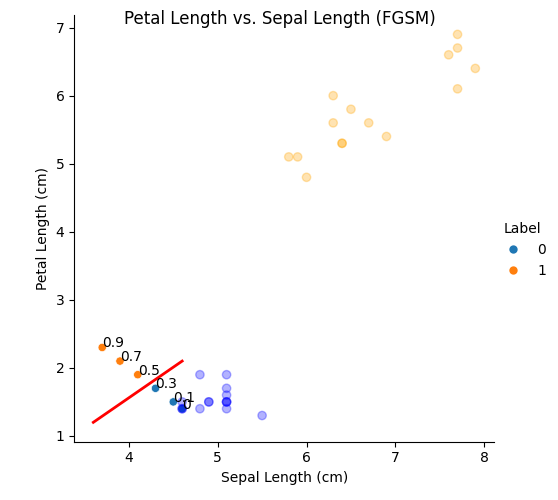
\includegraphics[scale=0.75]{figures/tabular-adversarial.png}
  \centering
  \caption{Effects of \ac{fgsm} on the Iris dataset's \textit{Petal Length} and \textit{Sepal Length} features for different attack strengths.}
~\label{fig:adversarial_tabular}
\end{figure} \

We can observe that the data point without any modifications
is classified with the label \(0\). With an increasing attack
strength the data point is modified such that the \textit{Sepal
Lenght} is reduced while the \textit{Petal Length} is increased.
The red line in this case represents the classification threshold,
where the \ac{qml} classifier starts labeling the data point as
\(1\) instead of \(0\). Once the features have been adapted
accordingly to exceed the classification threshold, the \ac{qml}
model will start to misclassify the data point. \

More significantly, we can still appreciate both clusters
formed by the data points and labels. We can observe that
the adversarial attack is significative, because the attacked
modified datapoints still don't come close to the cluster
with the \textit{real} label \(1\) while being misclassified.
Therefore, the attacked samples could still belong to the
cluster with the \textit{real} label \(0\). \

In the case of attacking a binary classificator, utilizing
a technique implementing an untargeted attack is equivalent
to executing a targeted attack aiming to obtain a misclassification
with the datapoint's contrary class. Therefore, for binary
classificators there is no distinction between performing a
targeted or an untargeted attack. However, this is not the case when
the \ac{qml} model is trying to differentiate between more than
two classes, as the result of an untargeted attack can now
be classified into more than one category. \

The attack strength regulates the magnitude of the perturbations
added to the original input to create the adversarial examples. 
In this thesis we chose \(5\) different attack strengths,
specifically the values \(\left[0.1, 0.3, 0.5, 0.7, 0.9\right]\).
This allows us to slowly increase the attack strength while
checking over a big range how the noisy and noiseless \ac{qml}
models react. Another factor that influenced this range is that
the attacks are being applied to the preprocessed data points
that have been normalized and rescaled. Nevertheless,
for the Plus-Minus dataset we had to adapt the attack
strength range and diminish the attack strength values to
\(\left[0.04, 0.08, 0.12, 0.16, 0.2\right]\).
The reason behind this new range is that the Plus-Minus
dataset has significantly more features than the previous
models, therefore, it is considerably easier to perform
the adversarial attacks. With the previous attack range
we would not see a smooth progression and it would drop to
almost 0\% after the first attack strength value of 0.1. \

\subsection{Automated Evaluation}\label{subsection:evaluation} \

Continuing the idea of the pipeline, evaluating the trained
\ac{qml} models should be simple to execute. The evaluation
requires two arguments, namely the dataset and a given \ac{qml}
model type to assess. The evaluation code will then
automatically calculate the accuracy scores of all the \(31\)
(Subsection~\ref{subsection:pipeline}) trained models. Additionally,
it also evaluates the \ac{qml} models against the two different
adversarial attacks with five differing attack strength.
The evaluation pipeline then results per dataset on \(341\)
data points to be analysed. \

In order to avoid performing a redundant assessment, first,
the pipeline will check if the evaluation and the figures
have already been created. If any of the two is missing,
the pipeline will automatically calculate the \ac{qml} models'
accuracies and draw the figures from the resulting data. To
do this, it verifies that all the adversarial samples have
already been crafted. \

The evaluation process iterates over all the noise
models (and its miscalibrations or noise probabilities)
and assesses each model with the modified adversarial
examples. The adversarial evaluation calculates first the
\ac{qml} model's accuracy against the unmodified test set.
Later on, the evaluation script retrieves the adversarial
examples for both adversarial attack techniques and their
variations and computes the adversarial accuracy of the model.
The results of this evaluation are saved in a file
for further use when creating the figures comparing the
accuracy of the different models in differents scenarios.
When the evaluation is performed, the weights of the noisy
models are retrieved, however, the evaluation is performed
with a noiseless model to stop the calculations from being
doubly impacted by the quantum noise. \

The resulting file from the evaluation process stores the
accuracies and the characteristics of the models. Per dataset,
we can retrieve \(31\) clean accuracies without any attack
performed and \(310\) adversarial accuracies, this corresponds
to the previously mentioned \(341\) number. This information
is required by the figure creation process. \

The graph creation process will output \(16\) different
figures belonging to \(2\) different types of graphs. Each
type of graph tries to convey a different comparison between
the different \ac{qml} models. The first type of graph deals
with the accuracy of the models on the clean dataset, 
with this graph we can observe the accuracy of the noiseless
model as well as how the noise probabilities or miscalibrations
affect the noisy models. \

In Figure~\ref{fig:sample-accuracy} we
can find a sample of this type of graphs, all the noise types
start at the \(0\) point on the \(x\)-axis with the same value. This
value represents the baseline performance of the noiseless model
on a chosen dataset. For the incoherent noise models, all the
noise models appear in one single graph to be able to also compare
them between each other. We separate the coherent noise model graphs
from the incoherent noise ones because the \(x\)-axis corresponds to
a different variable. \

\begin{figure}[h!]
  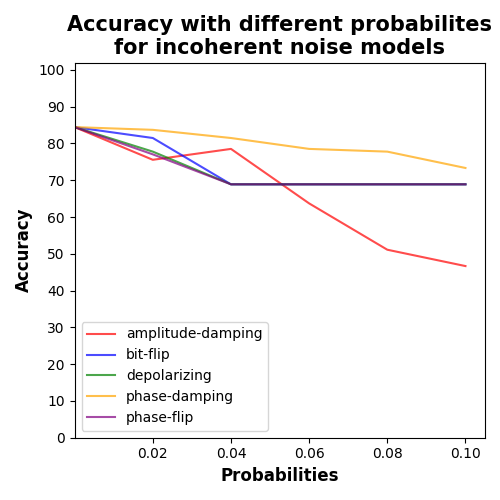
\includegraphics[scale=0.70]{figures/accuracy-graph.png}
  \centering
  \caption{Sample graph showing the effects on the model's accuracy of the noise probability modifications to the different noise models.}
~\label{fig:sample-accuracy}
\end{figure} \

The second type of graph can be found in Figure~\ref{fig:sample-adversarial}.
This graph demonstrates the changes that a given adversarial attack with
differing attack strengths provokes in the accuracy of differently trained
models. Thus, there is one graph per type of attack for each noise model,
which results in \(14\) graphs to be analyzed. The graphs for the
noiseless models are used to verify the effectiveness and the
correct working of both adversarial attack techniques. \

Furthermore, each graph has all the different variations of noise intensity
that affected during training each noise model. Additionally, the baseline
performance of the noiseless model can also be found with the \(0\) modification
label on the noisy graphs. Therefore, we can determine whether the noise
improves, decreases or doesn't modify the robustness of the trained \ac{qml}
models. \

\begin{figure}[h!]
  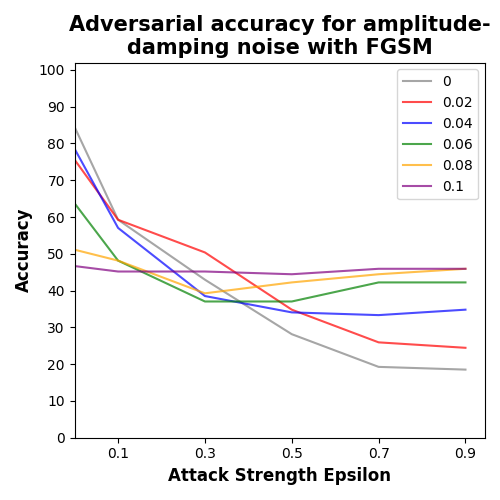
\includegraphics[scale=0.70]{figures/adversarial-graph.png}
  \centering
  \caption{Sample graph showing the effects on the model's accuracy of the attack strength modifications to the different noise models.}
~\label{fig:sample-adversarial}
\end{figure} \

With the automatic creation of the graphs we terminate the pipeline
for preprocessing, training, storing, attacking, and evaluating the
accuracy of noiseless and noisy \ac{qml} models. The pipeline implementation
reduces to the minimum the user interaction and allows us to automatically
perform the training of resource intensive \ac{qml} models. Additionally.
we can observe the effect of different types of noise and noise intensity
on model robustness against several adversarial attacks. Furthermore,
the pipeline allows us also to easily modify it by implementing new
architectures of \ac{qml} models or implementing new adversarial attack
techniques. Thus, further research of the effects of noise on \ac{qml}
model robustness is simple to perform. \
